We know present the results of the simulation under each environmental model.
Note that all simulations were run with the initial population frequencies \verb|[0.001,0.025,0.025,0.01,0.01,0.01,0.01,0.919]| (Table \ref{ft} order) and the following parameter values
% Parameter
\begin{table}[H]
    \centering
    $\begin{array}{lllllll}
        \toprule
        g_h & g_H & \mu_r & \mu_R & s_p & s_m & n  \\
        \midrule
        0.000001 & 0.00005 & 0.00001 & 0.00001 & 0.2 & 0.01 & 1000 \\
        \bottomrule
    \end{array}$
    \caption{Simulation parameter values.}
\end{table}
\FloatBarrier

The singular event models confirm that the model works as expected in response to events, although it appears that the antibiotic applies significantly more selective force on the population than the phage.
% Single Events
\FloatBarrier
\begin{figure}[htb!]
    \centering
    \begin{subfigure}[t]{0.45\textwidth}
        \centering
        \makebox[\textwidth][c]{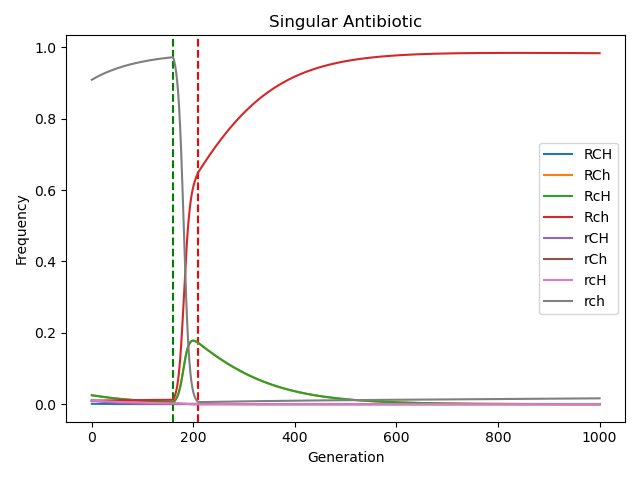
\includegraphics[width=\linewidth]{./figures/Singular_Antibiotic.png}}
        \caption{Single Antibiotic Event, event starts at green dotted line and ends at red dotted line.l=50}
    \end{subfigure}
    \begin{subfigure}[t]{0.45\textwidth}
        \centering
        \makebox[\textwidth][c]{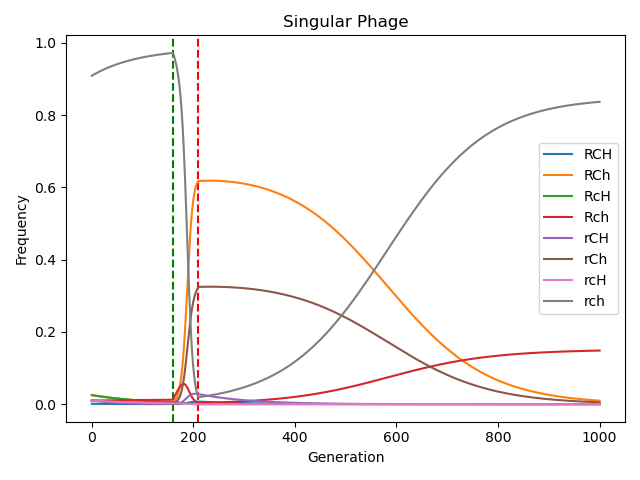
\includegraphics[width=\linewidth]{./figures/Singular_Phage.png}}
        \caption{Single Phage Event, event starts at green dotted line and ends at red dotted line. l=50}
    \end{subfigure}
    \caption{Single event simulations.}
\end{figure}
\FloatBarrier
With cyclical events, even with sustained selective pressure and a small metabolic cost that $C,H$ allele are quickly selected against relatively quickly.
We see undulations in the phage threat but unperturbed fixation with the antibiotic threat.
Since the $rCh,RCh$ are both the most fit genotypes in the cyclical phage environment it makes sense that they are the fixed alleles.
% Cyclical Events
\FloatBarrier
\begin{figure}[htb!]
    \centering
    \begin{subfigure}[t]{0.45\textwidth}
        \centering
        \makebox[\textwidth][c]{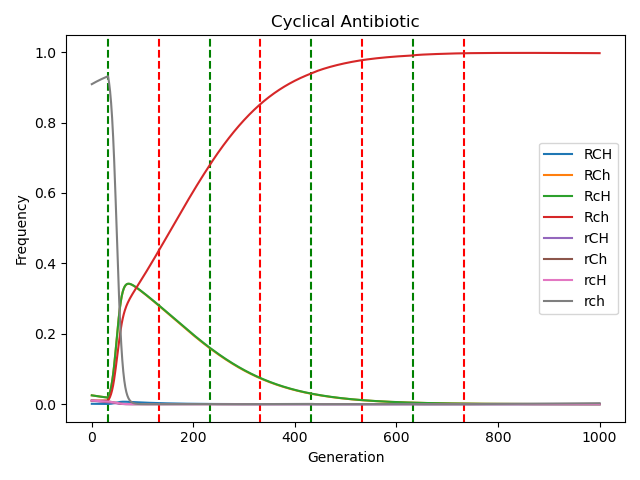
\includegraphics[width=\linewidth]{./figures/Cyclical_Antibiotic.png}}
        \caption{Cyclical Antibiotic Events, events start at green dotted line and ends at red dotted line. l=100}
    \end{subfigure}
    \begin{subfigure}[t]{0.45\textwidth}
        \centering
        \makebox[\textwidth][c]{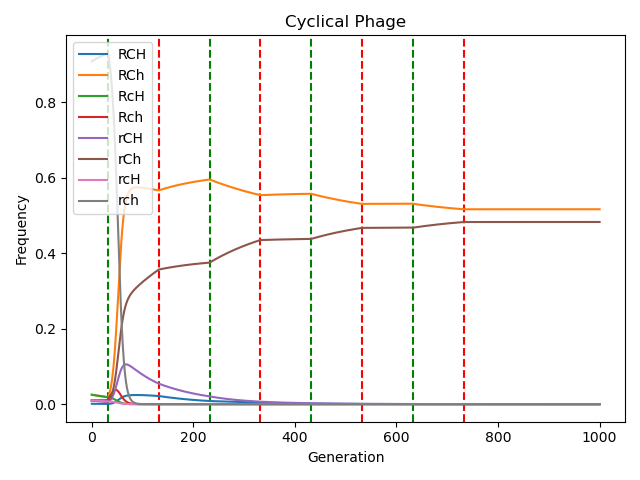
\includegraphics[width=\linewidth]{./figures/Cyclical_Phage.png}}
        \caption{Cyclical Phage Events, events start at green dotted line and ends at red dotted line. l=100}
    \end{subfigure}
    \caption{Cyclical event simulations.}
\end{figure}
\FloatBarrier
It is interesting to see the selective effect of the initial antibiotic breeding out most $r$ genotypes and then seeing further selection of $RC$ upon phage outbreak.
% Alternating Events
\FloatBarrier
% Cyclical Events
\FloatBarrier
\begin{figure}[htb!]
    \centering
    \begin{subfigure}[t]{0.45\textwidth}
        \centering
    \makebox[\textwidth][c]{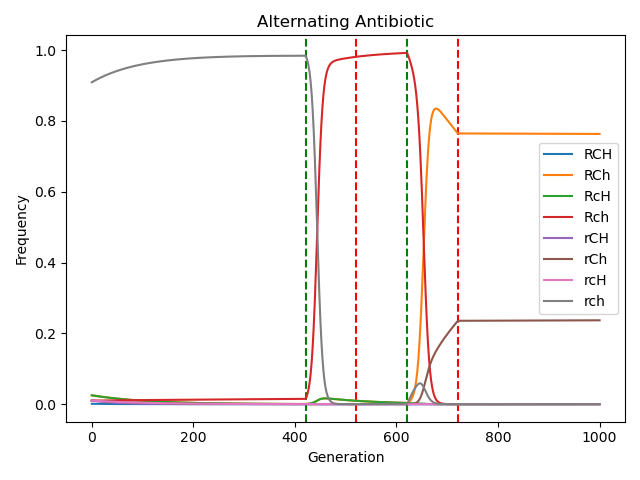
\includegraphics[width=\linewidth]{./figures/Alternating_Antibiotic.png}}
    \caption{Alternating Events, events start at green doted line and end at red dotted line, first event is Antibiotic. l=100}
    \end{subfigure}
    \begin{subfigure}[t]{0.45\textwidth}
        \centering
    \makebox[\textwidth][c]{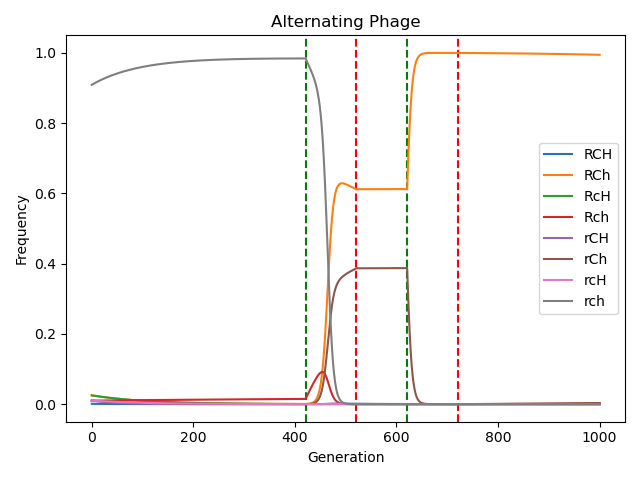
\includegraphics[width=\linewidth]{./figures/Alternating_Phage.png}}
    \caption{Alternating Events, events start at green doted line and end at red dotted line, first event is Phage. l=100}
    \end{subfigure}
    \caption{Alternating event simulations.}
\end{figure}
\FloatBarrier
The environmental stability show that no matter the frequency only a single dosage of antibiotic is enough to fix the $Rch$ genotype in the population.
However we see that the $RCh,rCh$ genotypes competing even under the alternating model for long turnover periods, but see fixation of $RCh$ with more consistent exposure to the antibiotic
% Stability Events
\FloatBarrier
\begin{figure}[htb!]
    \center
    \makebox[\textwidth][c]{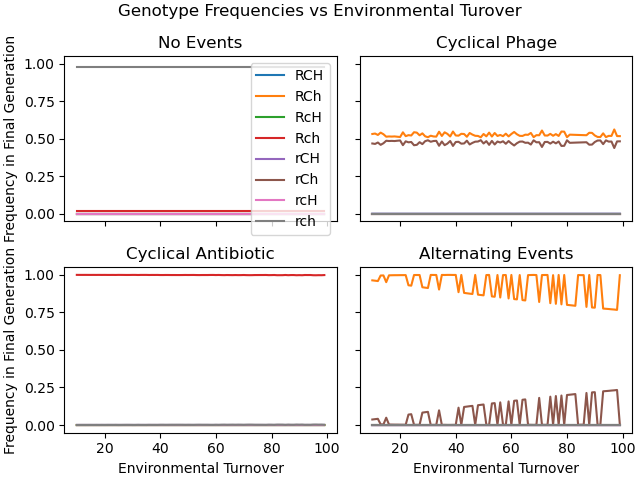
\includegraphics[width=\linewidth]{./figures/stability.png}}
    \caption{Environmental Stability, plot the genotypes frequencies in the 1000th generation for different event frequencies ($l$).}
\end{figure}
\FloatBarrier

\section{Discussion}
Ultimately I learn that a large part of defining a model is knowing where to create abstractions for simplicity.
\ac{crc} and \ac{hgt} are both highly complex and have unintuitive interactions so trying to include all of these interactions would results in too many parameters to examine and difficulty in understanding.

I also found that often parameter spaces for models need to be explored thoroughly.
Looking at how parameters vary with each other or what ranges of parameters can lead to chaotic behaviour are often the most interesting results from a paper.

Finally I realized the importance of defining parameters in your model such that they correspond nicely with the phenomena you are trying to study.
This helps with determining how studying the behaviour of the model can lead to interpretable conclusions about the phenomenon being studied.
